\chapter{Mutable Objects}
\label{mutable}

\index{String class}
\index{type!String}

As you learned in the previous chapter, an object is a collection of data that provides a set of methods.
For example, a \java{String} is a collection of characters that provides methods like \java{charAt} and \java{substring}.

In this chapter, we'll explore two new types of objects: \java{Point} and \java{Rectangle}.
We'll see how to write methods that take objects as parameters and produce objects as return values.

We will also take a first look at the source code for the Java library.


\section{Point Objects}
\label{point}

\index{coordinate}

In math, 2D ``points'' are often written in parentheses with a comma separating the coordinates.
For example, $(0,0)$ indicates the origin, and $(x,y)$ indicates the point $x$ units to the right and $y$ units up from the origin.

\index{AWT}
\index{java.awt}
\index{Point}
\index{class!Point}

% TODO: ML suggest introducing AWT here with a short high-level description

The \java{java.awt} package provides a class named \java{Point} that represents a location in a Cartesian plane.
In order to use the \java{Point} class, you have to import it:

\begin{code}
import java.awt.Point;
\end{code}

\index{new}
\index{operator!new}

Then, to create a new point, you use the \java{new} operator:

\begin{code}
Point blank;
blank = new Point(3, 4);
\end{code}

\index{declaration}
\index{statement!declaration}
\index{reference}

The first line declares that \java{blank} has type \java{Point}.
The second line creates the new \java{Point} with the coordinates $x=3$ and $y=4$.
The result of the \java{new} operator is a {\em reference} to the object.
%So \java{blank} contains a reference to the new \java{Point} object.
Figure~\ref{fig.reference} shows the result.

\index{memory diagram}
\index{diagram!memory}

\begin{figure}[!ht]
\begin{center}
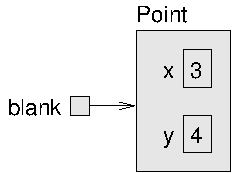
\includegraphics{figs/reference.pdf}
\caption{Memory diagram showing a variable that refers to a \java{Point} object.}
\label{fig.reference}
\end{center}
\end{figure}

As usual, the name of the variable \java{blank} appears outside the box, and its value appears inside the box.
In this case, the value is a reference, which is represented with an arrow.
The arrow points to the \java{Point} object, which contains two variables, \java{x} and \java{y}.


%\section{Attributes}

\index{attribute}
\index{dot notation}

Variables that belong to an object are called {\bf attributes}.
In some documentation, you also see them called ``fields''.
To access an attribute of an object, Java uses {\bf dot notation}.
For example:

\begin{code}
int x = blank.x;
\end{code}

The expression \java{blank.x} means ``go to the object \java{blank} refers to, and get the value of the attribute \java{x}.''
In this case, we assign that value to a local variable named \java{x}.

There is no conflict between the local variable \java{x} and the attribute \java{x}.
The purpose of dot notation is to identify {\em which} variable you are referring to unambiguously.

You can use dot notation as part of an expression.
For example:

\begin{code}
System.out.println(blank.x + ", " + blank.y);
int sum = blank.x * blank.x + blank.y * blank.y;
\end{code}

The first line displays \java{3, 4}.
The second line calculates the value \java{25}.


\section{Objects as Parameters}

\index{parameter}
\index{object!as parameter}

You can pass objects as parameters in the usual way.
For example:

\begin{code}
public static void printPoint(Point p) {
    System.out.println("(" + p.x + ", " + p.y + ")");
}
\end{code}

This method takes a point as an argument and displays its attributes in parentheses.
If you invoke \java{printPoint(blank)}, it displays \java{(3, 4)}.

As another example, we can rewrite the \java{distance} method from Section~\ref{distance} so that it takes two \java{Point}s as parameters instead of four \java{double}s.

\begin{code}
public static double distance(Point p1, Point p2) {
    int dx = p2.x - p1.x;
    int dy = p2.y - p1.y;
    return Math.sqrt(dx * dx + dy * dy);
}
\end{code}

Passing objects as parameters makes the source code more readable and less error-prone because related values are bundled together.

You actually don't need to write a \java{distance} method, because \java{Point} objects already have one.
To compute the distance between two points, we invoke \java{distance} on one and pass the other as an argument.

\begin{code}
Point p1 = new Point(0, 0);
Point p2 = new Point(3, 4);
double dist = p1.distance(p2);  // dist is 5.0
\end{code}

It turns out you don't need the \java{printPoint} method either.
If you invoke \java{System.out.println(blank)}, it prints the type of the object and the values of the attributes:

\begin{stdout}
java.awt.Point[x=3,y=4]
\end{stdout}

\index{toString}

\java{Point} objects provide a method called \java{toString} that returns a string representation of a point.
When you call \java{println} with objects, it {\em automatically} calls \java{toString} and displays the result.


\section{Objects as Return Values}
\label{sec:Rectangle}

\index{Rectangle}
\index{class!Rectangle}

The \java{java.awt} package also provides a class named \java{Rectangle}.
To use it, you have to import it:

\begin{code}
import java.awt.Rectangle;
\end{code}

\java{Rectangle} objects are similar to points, but they have four attributes: \java{x}, \java{y}, \java{width}, and \java{height}.
The following example creates a \java{Rectangle} object and makes the variable \java{box} refer to it:

\begin{code}
Rectangle box = new Rectangle(0, 0, 100, 200);
\end{code}

Figure~\ref{fig.rectangle} shows the effect of this assignment.

\begin{figure}[!ht]
\begin{center}
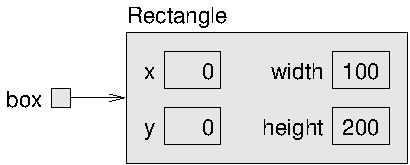
\includegraphics{figs/rectangle.pdf}
\caption{Memory diagram showing a \java{Rectangle} object.}
\label{fig.rectangle}
\end{center}
\end{figure}

If you run \java{System.out.println(box)}, you get:

\begin{stdout}
java.awt.Rectangle[x=0,y=0,width=100,height=200]
\end{stdout}

Again, \java{println} uses the \java{toString} method provided by \java{Rectangle}, which knows how to represent \java{Rectangle} objects as strings.

\index{return}
\index{statement!return}

You can also write methods that return new objects.
For example, \java{findCenter} takes a \java{Rectangle} as an argument and returns a \java{Point} with the coordinates of the center of the rectangle:

\begin{code}
public static Point findCenter(Rectangle box) {
    int x = box.x + box.width / 2;
    int y = box.y + box.height / 2;
    return new Point(x, y);
}
\end{code}

The return type of this method is \java{Point}.
The last line creates a new \java{Point} object and returns a reference to it.

%The \java{Rectangle} we created using the arguments \java{(0, 0, 100, 200)} has its upper-left corner in the origin.
%The center of this rectangle is \java{(50, 100)}, which is 50 pixels to the right and 100 pixels down from the origin.

\section{Rectangles are Mutable}

\index{mutable}
\index{object!mutable}

You can change the contents of an object by making an assignment to one of its attributes.
For example, to ``move'' a rectangle without changing its size, you can modify the \java{x} and \java{y} values:

\begin{code}
Rectangle box = new Rectangle(0, 0, 100, 200);
box.x = box.x + 50;
box.y = box.y + 100;
\end{code}

The result is shown in Figure~\ref{fig.rectangle2}.

\begin{figure}[!ht]
\begin{center}
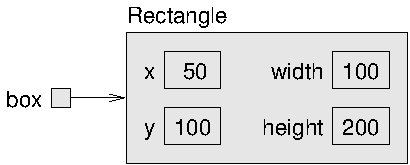
\includegraphics{figs/rectangle2.pdf}
\caption{Memory diagram showing updated attributes.}
\label{fig.rectangle2}
\end{center}
\end{figure}

\index{encapsulation}
\index{generalization}

We can encapsulate this code in a method and generalize it to move the rectangle by any amount:

\begin{code}
public static void moveRect(Rectangle box, int dx, int dy) {
    box.x = box.x + dx;
    box.y = box.y + dy;
}
\end{code}

The variables \java{dx} and \java{dy} indicate how far to move the rectangle in each direction.
Invoking this method has the effect of modifying the \java{Rectangle} that is passed as an argument.

\begin{code}
Rectangle box = new Rectangle(0, 0, 100, 200);
moveRect(box, 50, 100);  // now at (50, 100, 100, 200)
\end{code}

%The code displays \java{java.awt.Rectangle[x=50,y=100,width=100,height=200]}.

Modifying objects by passing them as arguments to methods can be useful.
But it can also make debugging difficult, because it is not always clear which method invocations modify their arguments.

Java provides a number of methods that operate on \java{Point}s and \java{Rectangle}s.
For example, \java{translate} has the same effect as \java{moveRect}, but instead of passing the rectangle as an argument, you use dot notation:

\begin{code}
box.translate(50, 100);
\end{code}

This line invokes the \java{translate} method on the object that \java{box} refers to, which modifies the object.

\index{object-oriented}

This syntax---using dot notation to invoke a method on an object, rather than passing it as a parameter---is more consistent with the style of object-oriented programming.


\section{Aliasing Revisited}
\label{aliasing}

\index{reference}

Remember that when you assign an object to a variable, you are assigning a {\em reference} to an object.
It is possible to have multiple variables that refer to the same object.
For example, this code creates two variables that refer to the same \java{Rectangle}:

\begin{code}
Rectangle box1 = new Rectangle(0, 0, 100, 200);
Rectangle box2 = box1;
\end{code}

Figure~\ref{fig.aliasing} shows the result: \java{box1} and \java{box2} refer to the same object, so any changes that affect one variable also affect the other.

\begin{figure}[!ht]
\begin{center}
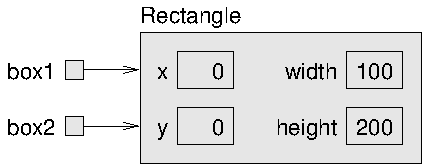
\includegraphics{figs/aliasing.pdf}
\caption{Memory diagram showing two variables that refer to the same \java{Rectangle} object.}
\label{fig.aliasing}
\end{center}
\end{figure}

For example, the following code uses \java{grow} to make \java{box1} bigger by 50 units in all directions.
It decreases \java{x} and \java{y} by 50, and it increases \java{height} and \java{width} by 100:

\begin{code}
box1.grow(50, 50);                // grow box1 (alias)
\end{code}

The result is shown in Figure~\ref{fig.aliasing2}.

\begin{figure}[!ht]
\begin{center}
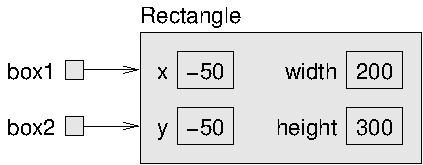
\includegraphics{figs/aliasing2.pdf}
\caption{Memory diagram showing the effect of invoking \java{grow}.}
\label{fig.aliasing2}
\end{center}
\end{figure}

Now, if we print \java{box1}, we are not surprised to see that it has changed.

\begin{code}
java.awt.Rectangle[x=-50,y=-50,width=200,height=300]
\end{code}

And if we print \java{box2}, we should not be surprised to see that it has changed, too, because it refers to the same object:

\begin{code}
java.awt.Rectangle[x=-50,y=-50,width=200,height=300]
\end{code}

This scenario is called ``aliasing'' because a single object has multiple names, or aliases, that refer to it.

As you can tell from this simple example, code that involves aliasing can get confusing fast, and it can be difficult to debug.


\section{Java Library Source}
\label{src.zip}

\index{library}
\index{source code}

So far we have used several classes from the Java library, including \java{System}, \java{String}, \java{Scanner}, \java{Math}, and \java{Random}.
These classes are written in Java, so you can read the source code to see how they work.

\index{src.zip}

The Java library contains thousands of files, many of which are thousands of lines of code.
That's more than one person could read and understand fully, but don't be intimidated!

Because it's so large, the library source code is stored in a ZIP archive named \java{src.zip}.
If you have Java installed on your computer, you should already have this file somewhere.

\begin{itemize}
\item On Linux, it's likely under: \verb"/usr/lib/jvm/.../lib"
\\ If not, you might have to install the {\tt openjdk-...-source} package.

\item On MacOS, it's likely under: \\ \verb"/Library/Java/JavaVirtualMachines/.../Contents/Home/lib"

\item On Windows, it's likely under: \verb"C:\Program Files\Java\...\lib"
\end{itemize}

When you open (or unzip) the file, you will see folders that correspond to Java packages.
For example, open the {\tt java} folder, and then open the {\tt awt} folder.
(If you don't see a {\tt java} folder at first, open the {\tt java.desktop} folder.)
You should now see {\tt Point.java} and {\tt Rectangle.java}, along with the other classes in the \java{java.awt} package.

Open {\tt Point.java} in your editor and skim through the file.
It uses language features we haven't discussed yet, so you probably won't understand every line.
But you can get a sense of what professional Java source code looks like by browsing through the library.

\index{documentation}
\index{HTML}
\index{Javadoc}

Notice how much of {\tt Point.java} is documentation (see Appendix~\ref{javadoc}).
Each method includes comments and tags like \java{@param} and \java{@return}.
Javadoc reads these comments and generates documentation in HTML.
You can see the same documentation online by doing a web search for ``Java Point''.

Now take a look at the \java{grow} and \java{translate} methods in the \java{Rectangle} class.
There is more to them than you may have expected.

% ABD: I'm not sure these conclusions follow from the example

%But that doesn't limit your ability to use these methods in a program.

%Object-oriented programming makes it possible to hide messy details so that you can more easily use and understand code that other people wrote.

%By looking at the source code for \java{Point}, \java{Rectangle}, and other classes, we hope you will learn two things.
%1) Objects encapsulate data and provide methods to access and modify the data directly.


\section{Class Diagrams}
\label{UML}

To summarize what we've learned so far, \java{Point} and \java{Rectangle} objects have attributes and methods.
Attributes are an object's {\em data}; methods are an object's {\em code}.
An object's {\em class} definition specifies the attributes and methods that it has.

\index{UML}

{\bf Unified Modeling Language} (UML) defines a graphical way to summarize this information.
Figure~\ref{fig.umlPoint}, shows two examples, the {\bf UML class diagrams} for the \java{Point} and \java{Rectangle} classes.

\begin{figure}[!ht]
\begin{center}
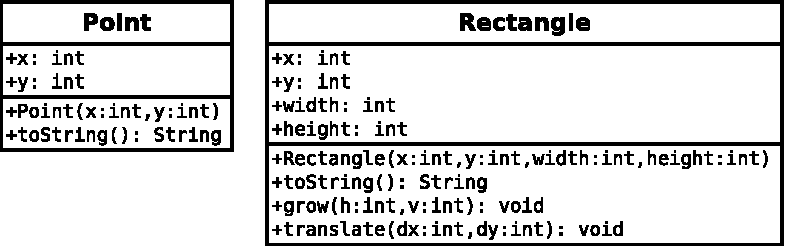
\includegraphics{figs/point-rect.pdf}
\caption{UML class diagrams for \java{Point} and \java{Rectangle}.}
\label{fig.umlPoint}
\end{center}
\end{figure}

\index{class diagram}
\index{diagram!class}

Each class is represented by a box with the name of the class,
a list of attributes, and a list of methods.

\index{private}
\index{variable!private}

To identify the types of attributes and parameters, UML uses a language-independent syntax, like {\tt x:~int} rather than Java syntax, \java{int x}.

The plus sign (\java{+}) identifies \java{public} attributes and methods.
A minus sign (\java{-}) identifies \java{private} attributes and methods, which we discuss in the next chapter.

Both \java{Point} and \java{Rectangle} have additional methods; we only show the ones introduced in this chapter.

In contrast to memory diagrams, which visualize objects (and variables) at run-time, a class diagram visualizes the source code at compile-time.


\section{Scope Revisited}

\index{scope}

In Section~\ref{stack}, we introduced the idea that variables have scope.
The scope of a variable is the part of a program where a variable can be used.

Consider the first few lines of the \java{Rectangle.translate} method from the Java library source code:

% TODO: ML suggests adding the header line of the class and the attribute declatrations 

\begin{code}
public void translate(int dx, int dy) {
    int oldv = this.x;
    int newv = oldv + dx;
    if (dx < 0) {
    ...
\end{code}

This example uses three kinds of variables:

\begin{enumerate}

\item Parameters (\java{dx} and \java{dy})

\item Local variables (\java{oldv} and \java{newv})

\index{this}

\item Attributes (\java{this.x})

\end{enumerate}

Parameters and local variables are created when a method is invoked, and they disappear when the method returns.
They can be used anywhere inside the method, but not in other methods and not in other classes.

Attributes are created when an object is created, and they disappear when the object is destroyed.
They can be used in any of the object's methods, using the keyword \java{this}.
And if they are public, they can be used in other classes via references to the object, \java{box1.x}.

When the Java compiler encounters a variable name, it searches backwards for its declaration.
The compiler first looks for local variables, then parameters, then attributes.

% ABD: The previous three paragraphs pack in a lot.  Some of it is a little early, and some of it is not explained carefully here.  So I think this is a soft spot to come back to in future revisions.


%\section{Shadowing}
%
% CSM: We now discuss shadowing in Chapter 11.
% @Deprecated is a nice idea, but unnecessary.
%
%It's possible to declare a local variable (or parameter) with the same name as an attribute.
%For example, you can declare \java{int x} in a method of the \java{Rectangle} class.
%In that method, the expression \java{x + 5} will refer to the local variable, even though there is an attribute named \java{x}.
%
%\index{shadowing}
%
%This situation is called {\bf shadowing}, because the local variable ``hides'' the attribute.
%Java provides the keyword \java{this} to refer to attributes explicitly.
%For example, look at the \java{Rectangle.reshape} method:
%
%\begin{code}
%@Deprecated
%public void move(int x, int y) {
%    this.x = x;
%    this.y = y;
%}
%\end{code}
%
%\index{scope}
%
%The variables \java{x} and \java{y} are parameters of the \java{move} method, and \java{this.x} and \java{this.y} are attributes of the rectangle being moved.
%These variables have the same name, but they have different scope.
%
%\index{deprecated}
%
%Notice that the \java{move} method has been {\bf deprecated}.
%Sometimes when new versions of Java are released, the library classes are revised or enhanced.
%The documentation for \java{Rectangle.move} indicates that the \java{setLocation} method should be used instead.
%
%The word ``deprecate'' means to express strong disapproval.
%Java discourages using deprecated methods, either because they are dangerous, or because better alternatives exist.
%The compiler will display a warning if you attempt to use a deprecated method.


\section{Garbage Collection}

In the previous section, we said that attributes exist as long as the object exists.
But when does an object cease to exist?
Here is a simple example:

%In Section~\ref{aliasing}, we saw what happens when more than one variable refers to the same object.
%What happens when {\em no} variables refer to an object?

\begin{code}
Point blank = new Point(3, 4);
blank = null;
\end{code}

The first line creates a new \java{Point} object and makes \java{blank} refer to it.
The second line changes \java{blank} so that instead of referring to the object, it refers to nothing.
As shown in Figure~\ref{fig.reference3}, after the second assignment, there are no references to the \java{Point} object.

% TODO: ML suggests revising this diagram to show before and after

\begin{figure}[!ht]
\begin{center}
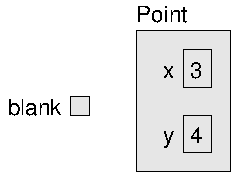
\includegraphics{figs/reference3.pdf}
\caption{Memory diagram showing the effect of setting a variable to \java{null}.}
\label{fig.reference3}
\end{center}
\end{figure}

If there are no references to an object, there is no way to access its attributes or invoke a method on it.
From the program's point of view, it ceases to exist.
However, it's still present in the computer's memory, taking up space.

\index{garbage collection}

As your program runs, the system automatically looks for stranded objects and deletes them; then the space can be reused for new objects.
This process is called {\bf garbage collection}.
%You can manually run the garbage collector by invoking \java{System.gc()} method.

You don't have to do anything to make garbage collection happen, and in general, you don't have to be aware of it.
But in high-performance applications, you may notice a slight delay every now and then while Java reclaims space from discarded objects.


\section{Mutable vs Immutable}

\index{mutable}
\index{immutable}

\java{Point}s and \java{Rectangle}s are {\bf mutable} objects, because their attributes can be modified.
You can modify their attributes directly, like \java{box.x = 15}, or you can invoke methods that modify their attributes, like \java{box.translate(15, 0)}.

In contrast, immutable objects like \java{String}s and \java{Integer}s cannot be modified.
They don't allow direct access to their attributes or provide methods that change them.

Immutable objects have a number of advantages that help improve the reliability and performance of programs.
You can pass strings (and other immutable objects) to methods without worrying about their contents changing as a ``side-effect'' of the method.
That makes programs easier to debug, and more reliable.

Also, two strings that contain the same characters can be stored in memory only once.
That can reduces the amount of memory the program uses, and can speed it up. 

% ABD: Do we want trinket markup in this version?  It seems to require cmplete class definitions, which involve code that's extraneous to the example.

In the following example, \java{s1} and \java{s2} are created differently, but they refer to equivalent strings; that is, the two strings contains the same characters.

\index{Surprise.java}

\begin{trinket}[265]{Surprise.java}
public class Surprise {
    public static void main(String[] args) {
        String s1 = "Hi, Mom!";
        String s2 = "Hi, " + "Mom!";
        if (s1 == s2) {                // true!
            System.out.println("s1 and s2 are the same");
        }
    }
}
\end{trinket}

Because both strings are specified at compile time, the compiler can tell that they are equivalent.
And because strings are immutable, there is no need to make two copies; the compiler can create one \java{String} and make both variables refer to it.

As a result, the test \java{s1 == s2} turns out to be true, which means that \java{s1} and \java{s2} refer to the same object.
In other words, they are not just equivalent; they are identical.

%Since neither variable can change the string itself, both \java{s1} and \java{s2} will be \java{"Hi, Mom!"} until they are reassigned.

Although immutable objects have some advantages, mutable objects have other advantages.
Sometimes it is more efficient to modify an existing object, rather than creating a new one.
And some computations can be expressed more naturally using mutation.

Neither design is always better, which is why you will see both.


\section{StringBuilder Objects}
\label{stringbuilder}

Here's an example where mutable objects are efficient and arguably more natural: building a long string by concatenating lots of small pieces.

Strings are particularly inefficient for this operation.
For example, consider the following program, which reads ten lines from \java{System.in} and concatenates them into a single \java{String}.

\index{Append.java}

\begin{code}
String text = "";
for (int i = 0; i < 10; i++) {
    String line = in.nextLine();        // new string
    text = text + line + '\n';    // two more strings
}
\end{code}

Inside the \java{for} loop, \java{in.nextLine()} returns a new string each time it is invoked.
The next line of code concatenates \java{text} and \java{line}, which creates another string, and then appends the newline character, which creates yet another string.

As a result, this loop creates 30 \java{String} objects!
At the end, \java{text} refers to the most recent \java{String}.
Garbage collection deletes the rest, but that's a lot of garbage for a seemly simple program.

\index{StringBuilder}

The Java library provides the \java{StringBuilder} class for just this reason.
It's part of the \java{java.lang} package, so you don't need to import it.
Because \java{StringBuilder} objects are mutable, they can implement concatenation more efficiently.

Here's a version of the program that uses \java{StringBuilder}:

%TODO: ML suggests also showing how to print the results

\begin{code}
StringBuilder text = new StringBuilder();
for (int i = 0; i < 10; i++) {
    String line = in.nextLine();
    text.append(line);
    text.append('\n');
}
\end{code}

The \java{append} method takes a \java{String} as a parameter and appends it to the end of the \java{StringBuilder}.
Each time it is invoked, it modifies the \java{StringBuilder}; it doesn't create any new objects.

The \java{StringBuilder} class also provides methods for inserting and deleting parts of strings efficiently.
Programs that manipulate large amounts of text run much faster if you use \java{StringBuilder} instead of \java{String}.


\section{Vocabulary}

\begin{description}

\term{attribute}
One of the named data items that make up an object.
%Each object has its own copy of the attributes for its class.

\term{dot notation}
Use of the dot operator (\java{.}) to access an object's attributes or methods.

\term{UML}
Unified Modeling Language, a standard way to draw diagrams for software engineering.

\term{class diagram}
An illustration of the attributes and methods for a class.

%\term{deprecated}
%A library method that has been replaced by another method, but left in the class for backwards compatibility.

\term{garbage collection}
The process of finding objects that have no references and reclaiming their storage space.

\term{mutable}
An object that can be modified at any time.
Points and rectangles are mutable by design.

\end{description}


\section{Exercises}

The code for this chapter is in the {\tt ch10} directory of {\tt ThinkJavaCode2}.
See page~\pageref{code} for instructions on how to download the repository.
Before you start the exercises, we recommend that you compile and run the examples.

At this point you know enough to read Appendix~\ref{graphics}, which is about simple 2D graphics and animations.
During the next few chapters, you should take a detour to read this appendix and work through the exercises.


\begin{exercise}  %%V6 Ex10.1

The point of this exercise is to make sure you understand the mechanism for passing objects as parameters.

\begin{enumerate}

\item For the following program, draw a stack diagram showing the local variables and parameters of \java{main} and \java{riddle} just before \java{riddle} returns.
Use arrows to show which objects each variable references.

\item What is the output of the program?

\item Is the \java{blank} object mutable or immutable?
How can you tell?

\end{enumerate}

\begin{code}
public static int riddle(int x, Point p) {
    x = x + 7;
    return x + p.x + p.y;
}
\end{code}

\begin{code}
public static void main(String[] args) {
    int x = 5;
    Point blank = new Point(1, 2);

    System.out.println(riddle(x, blank));
    System.out.println(x);
    System.out.println(blank.x);
    System.out.println(blank.y);
}
\end{code}

\end{exercise}


\begin{exercise}  %%V6 Ex10.2

The point of this exercise is to make sure you understand the mechanism for returning new objects from methods.
The following code uses \java{findCenter} and \java{distance} as defined in this chapter.

\begin{enumerate}

\item Draw a stack diagram showing the state of the program just before \java{findCenter} returns.
Include all variables and parameters, and show the objects those variables refer to.

\item Draw a stack diagram showing the state of the program just before \java{distance} returns.
Show all variables, parameters, and objects.

\item What is the output of this program?
(Can you tell without running it?)

\end{enumerate}

\begin{code}
public static void main(String[] args) {
    Point blank = new Point(5, 8);

    Rectangle rect = new Rectangle(0, 2, 4, 4);
    Point center = findCenter(rect);

    double dist = distance(center, blank);
    System.out.println(dist);
}
\end{code}

\end{exercise}


\begin{exercise}  %%V6 Ex10.3

This exercise is about aliasing.
Recall that aliases are two variables that refer to the same object.
The following code uses \java{findCenter} and \java{printPoint} as defined in this chapter.

\begin{enumerate}

\item Draw a diagram that shows the state of the program just before the end of \java{main}.
Include all local variables and the objects they refer to.

\item What is the output of the program?

\item At the end of \java{main}, are \java{p1} and \java{p2} aliased?
Why or why not?

\end{enumerate}

\begin{code}
public static void main(String[] args) {
    Rectangle box1 = new Rectangle(2, 4, 7, 9);
    Point p1 = findCenter(box1);
    printPoint(p1);

    box1.grow(1, 1);
    Point p2 = findCenter(box1);
    printPoint(p2);
}
\end{code}

\end{exercise}
